\section{ARIFI's project description}
ARIFI is an ongoing project whose main goal is to combine GNSS services with Artificial intelligence into a web application. This application will provide agricultors not only with useful data, but also with instructions on what actions to take so as to manage more efficiently their farms and improve their harvest profits.\\
%
%
The project started after a several discussions with farmers from different countries around the world. Amongst all the professionals we reached, we established tighter connection with the ones presented in section \ref{adv}, which up to this day constitute our advisory board. The intention of all the conversations via phone calls or e-mail, was to get a deeper insight on the state of the art concerning agriculture. We tried to analyse common difficulties among farmers, despite being far apart from one another, making special emphasis in those that we thought we could contribute to, as a team with solid knowledge in GNSS and AI.\\
%
%
In conclusion, we obtained valuable feedback from farmers that helped the team to better shape the project and define more clearly which difficulties we wanted to address with ARIFI. The latter have been itemised and briefly described next, so as to give a more schematic look of what we concluded.
% REVISAAAAAAAAAAAAAAR JOAN
%::::::::::::::::::
%::::::::::::::::::
%::::::::::::::::::
\begin{itemize}
    \item \textbf{Interpretation of weather forecasts:} It is well known that weather forecasts are of extreme importance for agriculture. It helps farmers to prevent their harvest to be damaged and also to adjust farming systems that perform vital functions such as irrigation. In this concrete aspect, we found
    that in the first place, farmers received weather forecasts, either on their own or by means of external companies, that where not detailed enough in many cases. In the second place and more importantly, most of these forecasts were only useful for well experienced agricultors, who knew to interpret this data and deduct what actions to take in consequence. This is a problem that ARIFI wants to solve, not only by providing more detailed weather forecasts, but also to combine them with data from other sources so as to provide farmers with instructions on how to proceed with their farming activities. We want to make from ARIFI an ally for a wide range of farmers, whatever their technical knowledge or work experience. Plus, we think ARIFI can be specially useful in developing countries' agricultural sector, where consulting services from specialised companies are limited. 
    \item \textbf{knowledge of field's characteristics:} Although all farmers know their fields to some extend, not many have precise and/or detailed knowledge about more concrete aspects aspects, e.g. soil height irregularities, chemical characteristics etc. These parameters should be taken into account in order to optimise many farming activities. The major handicap in this aspect is that they are not easy to determine, and in some cases it implies an expensive and time-consuming deployment of measuring devices. ARIFI expects to contribute to this necessity by offering farmers more detailed knowledge of their farms, making use of GNSS services combined with AI and signal/image processing techniques.
    \item \textbf{Adaptation to climate change:} Climate change affects agriculture in particular by changing the intensity and duration of certain meteorologic conditions. This not only affects the way farmers have to manage their fields, but also shifts periodic climate conditions within the year, which threats agricultors' farming schedules. That being said, to optimise their harvest, farmers should not only anticipate threatening climate changes, such as heat waves, but also to adapt their yearly farming schedule to these climate shifts.
    ARIFI aims to provide support to farmers in this issue by making thanks to its artificial intelligence module. The latter will keep track of climate distortions over time so as to make more accurate predictions of climate changes and shifts.  
\end{itemize}
As mentioned earlier, ARIFI is an ongoing project under development. Even though its main objectives are well outlined at the moment, thanks to the potential of the technical subjects in which it is based (GNSSs and AI), it has the potential of being a very scalable project, which will be able to adapt and introduce new features in the future.

\subsection{Project overview}
%
\begin{figure}[b!]
    \centering
    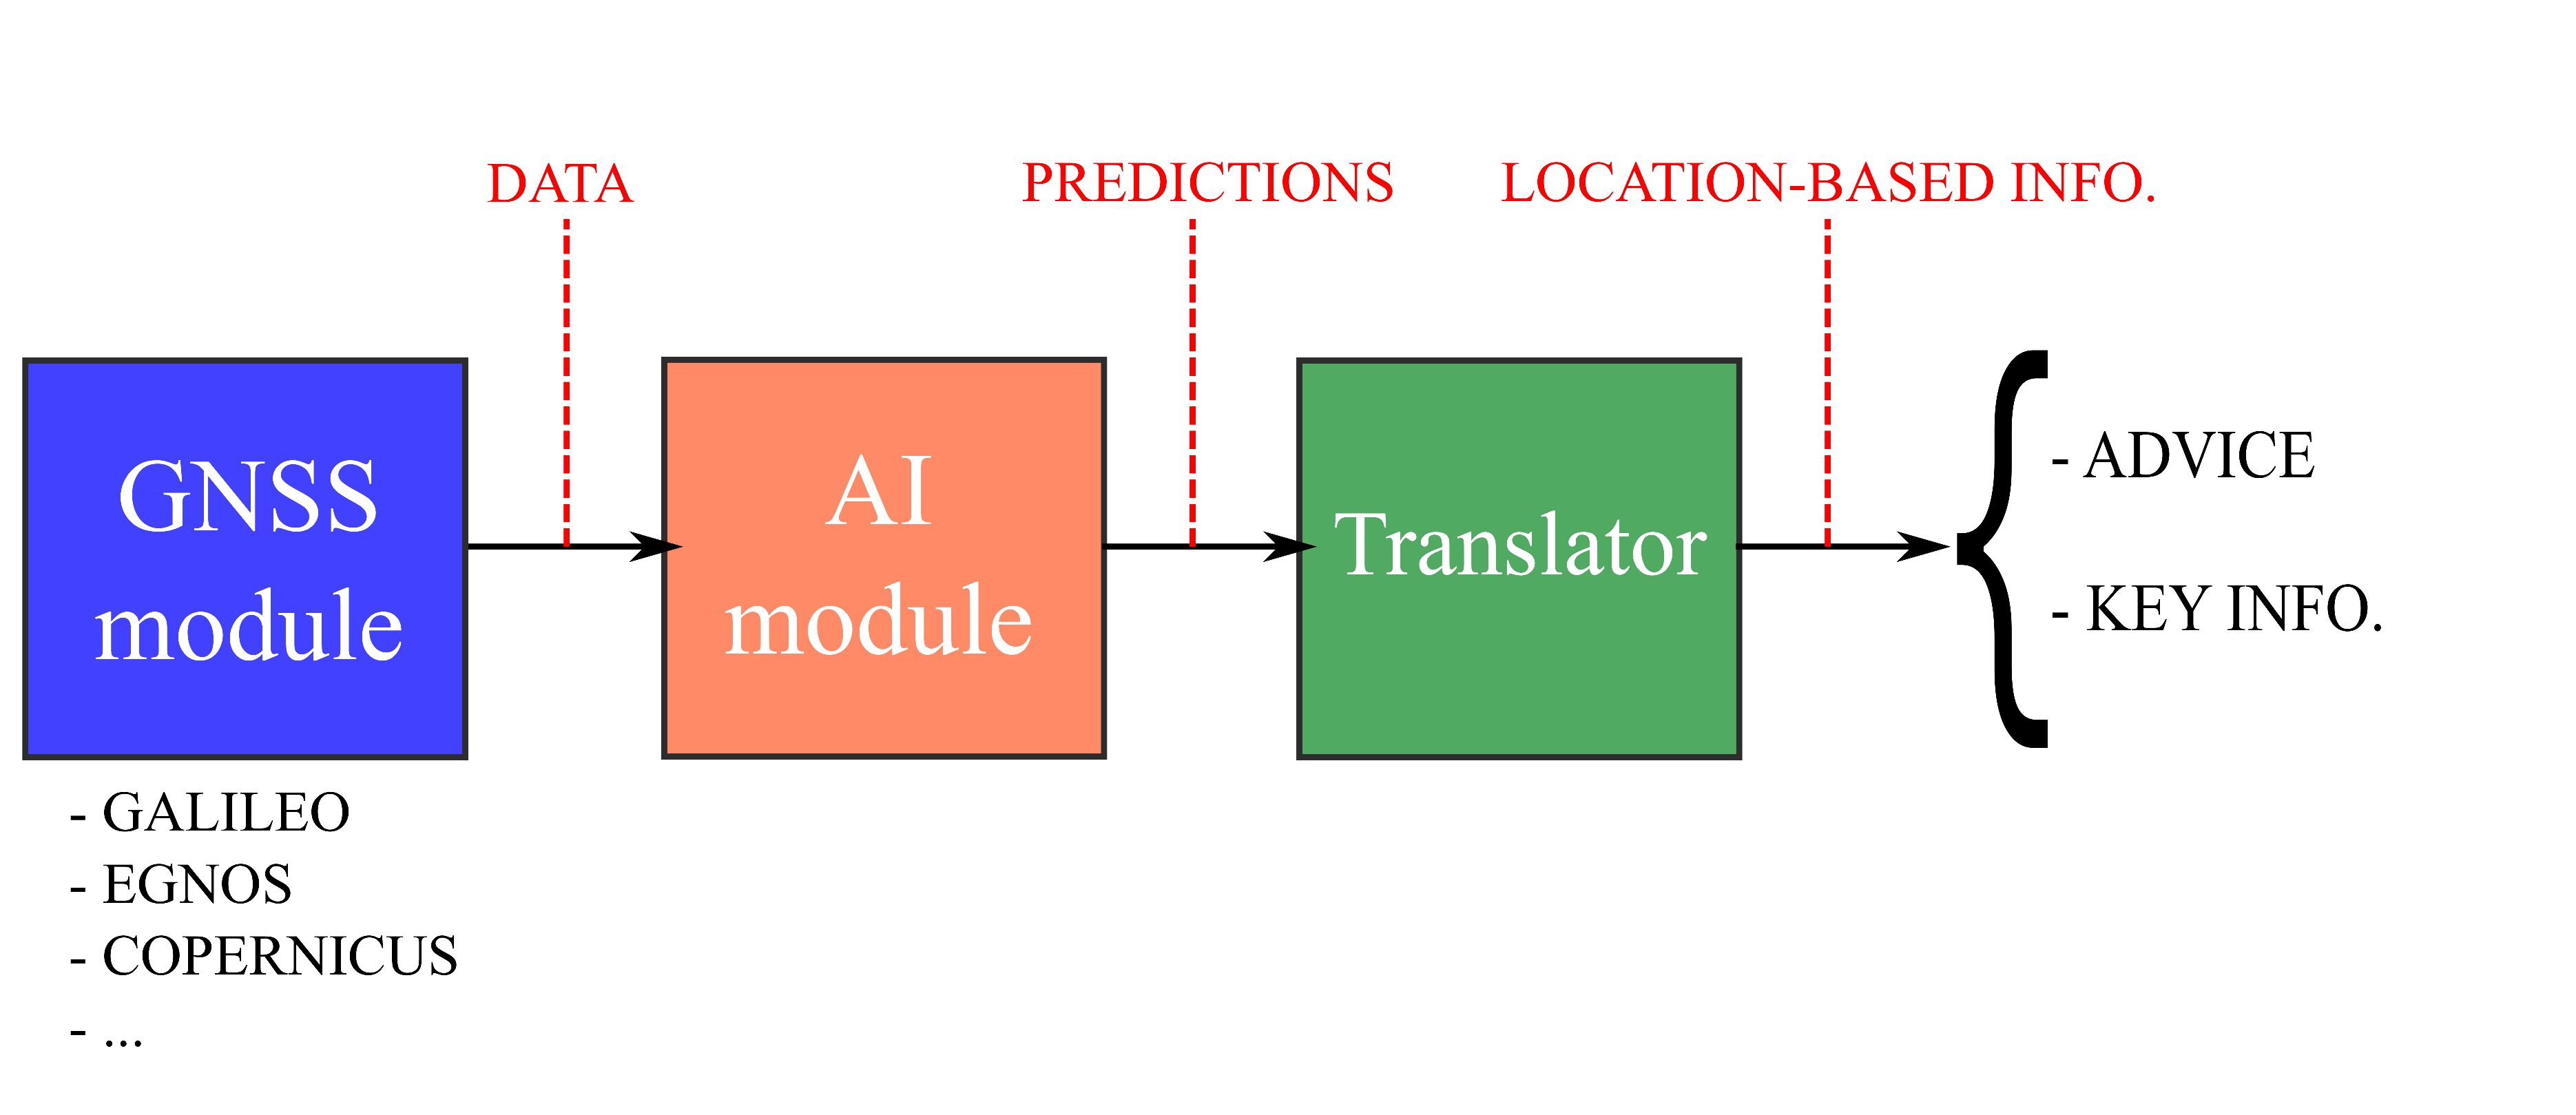
\includegraphics[scale= 0.26]{images/dibujo1.eps}
    \caption{ARIFI's general schematic}
    \label{fig:sch1}
\end{figure}
%
The principal idea is that GNSS together with other sources act as data providers to ARIFI's AI module, which will collect and integrate this information to its algorithm. Next, the AI module will output a prediction of key parameters, that will be later interpreted and made understandable for agricultors. This part is where ARIFI specially stands out from other services, as it will make special emphasis in translating AI predictions into instructions for farmers, so that their harvest follows a more efficient agricultural plan. In figure \ref{fig:sch1}, it is displayed an schematic idea of ARIFI's general concept.\\\\
%
\begin{figure}[t!]
    \centering
    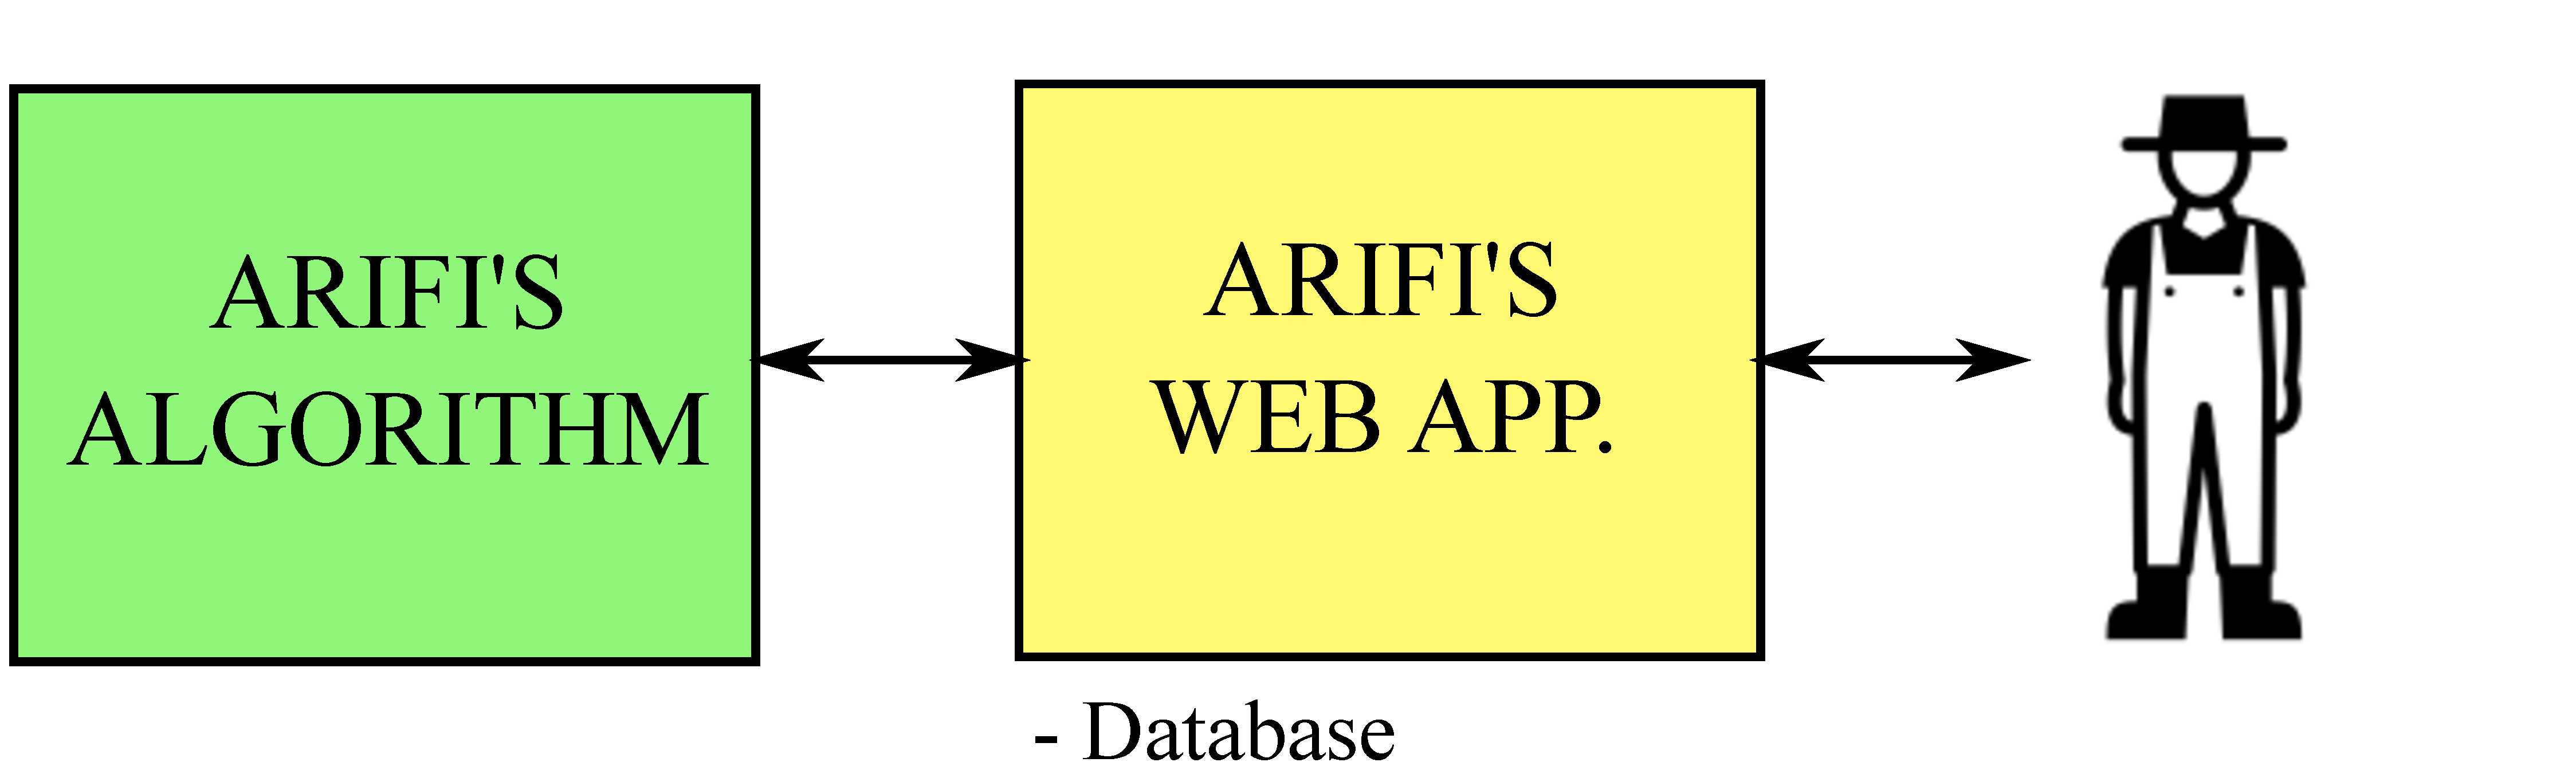
\includegraphics[scale= 0.15]{images/dibujo2.eps}
    \caption{User interaction with ARIFI's services}
    \label{fig:sch2}
\end{figure}
%
ARIFI was initially thought to work as a web application. The reason to this is that one of the major concerns from ARIFI's team, was to make this service available for a wide range of users. With this in mind, a web application was thought the best platform to work with, as it only requires a device with internet connection to access to its services. Despite this, we are opened to consider other platforms such as mobile-phone applications in the future. A graphical description of user's interaction with ARIFI is depicted in figure \ref{fig:sch2}.

\newpage
\subsection{Technical aspect}
\subsubsection{Satellite services}
\begin{itemize}
    \item \textbf{GALILEO}
    \item \textbf{EGNOS}
    \item \textbf{Copernicus}
    
\end{itemize}
\subsubsection{Artificial intelligence}
To address the proposed idea and achieve our goal, we will focus on how to relate machine learning techniques, field of Artificial Intelligence (AI), with the study of the atmosphere provided by satellite data. Thanks to the Copernicus Atmosphere Monitoring Service, we will be able to access to data that will allow us to predict the main atmospheric phenomenons which affects the production of the majority farmers.\\\\
%
In particular, we are talking about reanalysis variables. This kind of data is obtained by some weather forecasting centres, which combine past observations with a modern meteorological forecast model, in order to produce regular gridded datasets of many atmospheric and oceanic variables, with a temporal resolution of a few hours. This datasets usually extend over several decades and cover the entire planet, being a very useful tool for meteorological and climatological studies.\\\\
%
One of the most important reanalysis projects is the {\em ERA-Interim reanalysis project}, produced by the European Centre for Medium-Range Weather Forecasts (ECMWF) \cite{ERA_Interim}, which belongs to the Copernicus Programme. ERA-Interim is a global atmospheric reanalysis from 1979, continuously updated in real time.\\\\
%
Table \ref{Variables_ERA} is just an example of variables that can be obtained from this platform, which could be used as predictors in machine learning models.

\vspace{12pt}
\begin{table}[H]
\begin{center}
\caption{\label{Variables_ERA} Possible predictive variables in a prediction problem.}
\begin{tabular}{cccc}
\hline
variable name & ERA-Interim variable\\
\hline
\hline
skt & surface temperature\\
sp & surface pression\\
$u_{10}$& zonal wind component ($u$) at 10m\\
$v_{10}$& meridional wind component ($v$) at 10m\\
temp1& Temperature at 500hPa\\
up1& zonal wind component ($u$) at 500hPa\\
\hline
\end{tabular}
\end{center}
\end{table}
\vspace{12pt}

Due to the chaotic nature of atmospheric phenomenons it is so difficult predict with precision its future state. Modeling it without any un- certainty is not possible as there is a strong sensitivity to small perturbations in the initial conditions. But there is a way to overcome this issue by the use of probabilistic weather forecasts \cite{martinez2015forecasting}. In this regard, we propose computational methods belonging to machine learning techniques, a branch of AI, to get predictions or classifications over the main atmospheric factors with high accuracy. We could predict solar radiation, wind velocity, or whatever meteorological process that injures in the farmers' environment. Of course, it would not be possible without GNSS services that provide the essential dataset, as we mentioned before, necessary to train the learning models.

Many of these methods can be classified in the field of Knowledge called “Natural Computing”. The algorithms that can be found in this category are inspired by the way Nature solves complex problems. In this regard, Evolutionary Computation (EC) is inspired in the theory of evolution or Artificial Neural Networks (ANN) find their behaviour in human brain.

The conjunction between satellite data and machine learning algorithms will allow us to provide solutions to those aspects that most concern farmers, in order to keep their harvests safe with the highest possible productivity. For instance, if we are able to anticipate how much water they will have at a given time, or to warn of a dry season that was not previously contemplated but, due to the effects produced by climate change may occur, we will have a positive influence on their economy by avoiding unnecessary expenses derived from poor management, because they do not have all the information they could.

\subsubsection{Comparisons}	
The beginning of a project takes place after analysing the subject's state of the art to which it addresses. In this research, it is important to determine that the development of the project's idea will bring added value with respect to already existing solutions. In ARIFI, we have relied on our supervisors, who are well familiarised with agriculture topics, to know from first hand some of the real necessities farmers have, and how are they currently faced, assuming they are. The intention of this section is to make a more detailed comparison between the approeach of ARIFI and methods that are currently being used to overcome the difficulties presented in section X. We will recover them and make a brief comparison in the following bullet-points. 
\begin{itemize}
    \item \textbf{Interpretation of weather forecasts:} 
    \item \textbf{knowledge of field's characteristics:} 
    \item \textbf{Adaptation to climate change:} 
\end{itemize}

\subsection{Discussion of critical areas}
\subsection{Schedule}
